\chapter{Body}
\thispagestyle{pagestyle}

\section{FIGURES AND PHOTOGRAPHS}

Figures (including images, graphs and screenshots) are numbered in order of their appearance in the paper. Alternatively, figures may be numbered in order in each chapter, including the chapter number. Each figure has a number and a title, which is mentioned under the figure, centered. Where applicable, the source of the figure shall be indicated in brackets after the title of the figure;

All figures and photographs inserted in the paper must be referenced in the text, numbered and titled.

There will be a blank line (Nimbus Sans 12 pt) between the figure and the text. Figures will be centered.

\begin{figure}[h]
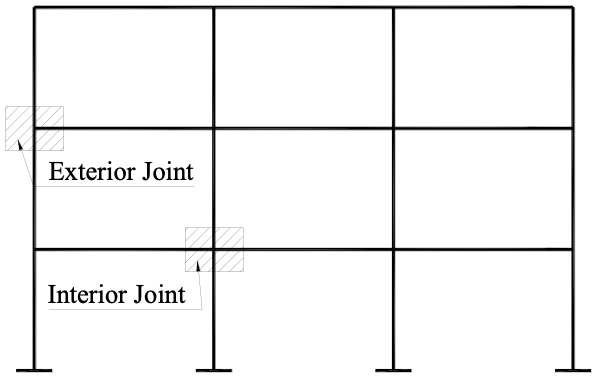
\includegraphics{images/Picture 1.png}
\caption{Example of a figure (source: The Scientific Bulletin of the UPT – series Building Engineering – Architecture, issue 2/2010)}
\label{fig:myfig}
\end{figure}

A reference to a figure can be created: \cref{fig:myfig}. 

\section{TABLES}

Tables will be numbered in the order in which they appear in the paper. Alternatively, tables can be numbered in order in each chapter, including the chapter number in the numbering. Each table has a number and a title, which is mentioned above the table, in a centered alignment. Where applicable, the data source shall be indicated in brackets after the title of the table.

All tables presented in the paper must be referenced in the text of the paper, must be numbered and accompanied by a title (see example below). If copied figures are used, the source of the photo will be indicated in parenthesis. As far as possible, the usual font (Nimbus Sans 12 pt) will be kept in the table, but there are also accepted ways to highlight important results (Bold, Italics, etc.)

A blank line (Nimbus Sans 12 pt) will be left between the text and the table. Tables will be centered. 

\begin{table}[h]
\caption{Example of a table}
\label{table:table1}
\begin{tabular}{ |p{2.9cm}|p{2cm}|p{3cm}|p{2cm}|p{3cm}|  }
 \hline
  &  \multicolumn{2}{|c|}{Yield stress, fy [N/mm2]} & \multicolumn{2}{|c|}{Tensile strength, fu [N/mm2]} \\
 \hline
 Element & Mill certificate & Coupon tests & Mill certificate & Coupon tests \\
 \hline
 Beam IPE360 & 285.0 & 329.8 flange 348.4 web & 427.0 & 463.2 flange 464.0 web \\
 \hline
 Column HEB300 & 311.3 & 313.0 flange 341.8 web	& 446.0	& 449.8 flange 464.4 web \\
 \hline
 End plate & 281.0 & 248.3 & 424.7 & 416.0 \\
 \hline
 Cover plate & 296.0 & 273.2 & 443.0 & 436.7 \\
 \hline
\end{tabular}
\end{table}


A reference to a table can be created: \cref{table:table1}. To create a table, one can use \label{example:table_url} \url{https://www.tablesgenerator.com/latex_tables}.

\section{FORMULAE}

Formulas used in the text will be numbered in order of appearance in the paper. Alternatively, formulas can be numbered in order in each chapter, including the chapter number. The numbering of formulas is done in round brackets. A blank line (arial 12 pt) will be left between the text and the formula. Formulas will be aligned to the right.
\begin{equation}
\label{eq:myeq}
A=\pi r^2
\end{equation}
A reference to an equation can be created: \cref{eq:myeq}. 

\section{CODE}

\begin{code}
	\begin{lstlisting}[language=Java]
public class Client {
    public static void main(String[] args) {
        Animal tiger = new Tiger();
        Animal parrot = new Parrot();
        tiger.breed(parrot);
    }
}
	\end{lstlisting}
	\caption{Subtype polymorphism example \cref{code:polym}}
	\label{code:polym}
\end{code}
Flexibility introduced by polymorphism can be seen in \cref{code:polym}, lines \textit{(3)}, \textit{(4)}. Variables, \texttt{tiger} and \texttt{parrot}, baing of type \texttt{Animal}, can refer to \texttt{Tiger}, or \texttt{Parrot} objects. Still, this flexibility becomes a problem when dealing with call such as that in line \textit{(5)}, since „breeding” makes sense only between objects having the same type.

\begin{code}[H]
	\begin{lstlisting}[language=Java]
public class Client {
	public static void main(String[] args) {
		Animal tiger = new Tiger();
		Animal parrot = new Parrot();
		tiger.breed(parrot);
	}
}
	\end{lstlisting}
	\caption{Subtype polymorphism example \cref{code:polym}}
	\label{code:polym2}
\end{code}